
% !TEX root = TD_fluides_part1.tex


\appendix
\section{Exercices de synthèses et annales d'examens}





\subsection{Vitesse de gouttes et particules en chute libre (partiel 2017)}

%\section{Vitesse de gouttes et particules en chute libre}

On considère une particule sphérique $ {\cal S}$ de rayon $a$, volume $V = 4 \pi a^3/3$
et masse volumique $\rho_p$ qui se déplace verticalement sous l'effet de la gravité $g$ dans un fluide ${\cal F}$ de viscosité dynamique $\mu$ et masse volumique $\rho_f$ supposée uniforme.  

On cherche à estimer la vitesse finale $U$ de celle-ci ainsi que le temps caractéristique 
$[T] =  \tau$ au bout duquel cette vitesse est atteinte en supposant qu'elle est lâchée à vitesse initiale nulle à l'instant $t=0$.

\begin{enumerate}

\item Ecrire les équations de Navier-Stokes sous une forme faisant
intervenir la pression motrice $\hat{p} = p + \rho_f g z$. Quelle est l'interprétation ce cette quantité ?

\item Donnez l'expression générale, sous forme d'une intégrale, de la force exercée par le fluide sur la surface de la sphère, puis montrez que celle-ci peut se décomposer sous la forme suivante :
$$
\vec F_{{\cal F} -> {\cal S}} = \vec F_A + \vec F_h  \mbox{ avec } 
\vec F_A = - \rho_f g V \vec e_z  
\mbox{ et } 
\vec F_h
= \int_{\cal S} \left( -\hat{p} \vec n + \mytensor{\tau } \cdot \vec n \right) dS
$$
Quelle est l'interprétation respective des deux termes $\vec F_A$ et $ \vec F_h$ ?

%\begin{enumerate}
%\itùem
%\end{itemize}

\item
Donnez l'ordre de grandeur des 4 différents termes de l'équation de Navier-Stokes écrite à la question 1. 
(On notera $[\hat p]$ l'ordre de grandeur des variations de pression motrice au sein du fluide).


\item En comparant l'ordre de grandeur du terme visqueux et du terme convectif, donnez la condition, faisant intervenir un nombre sans dimension classique, pour laquelle ce second 
terme peut être négligé.

On supposera dans la suite cette condition satisfaite.

\item A l'aide du principe de moindre dégénérescence, donnez l'ordre de grandeur de la jauge de pression $[\hat p]$ et de l'échelle de temps $[T]$. Quelle échelle de temps caractéristique reconnait-on dans cette dernière expression ?

\item Justifiez que l'ordre de grandeur du terme $\vec F_h$ vaut :
$$
[F_h]  \approx \mu a  U
$$
Que peut-on dire des contributions respectives de la pression motrice et de la contrainte visqueuse?
%exercée sur une particule sphérique est $F_z = 6 \pi \mu a  U$.



\item  
%Par un raisonnement dimensionnel, justifiez la forme de cette expression (on ne demande pas de démontrer le facteur $6\pi$). 
La résolution exacte des équations de Stokes autour d'une sphère permet de montrer le résultat suivant, que l'on admettra dans la suite :

$$|\vec F_h| = 6 \pi \mu a  U.$$


%\item
 Par un bilan des forces exercées sur la particule (son poids et la force exercée par le fluide exprimée selon la décomposition de la question 2), déterminez la vitesse de la particule prédite par cette formule dans les 4 cas suivants :

$(a)$ Gouttelette de brouillard ($a = 10 \mu m$, $\rho_p = 1000kg/m^3$) en chute dans de l'air ($\rho_f = 1.225 kg/m^3, \nu = 1.5\cdot 10^{-5} m^2/s$).

% Réponse : $U = 1.2 cm/s$ ; $Re = 7 \cdot 10^{-3}$.

%$(b)$ Bulle d'air ($a = 0.1mm$, $\rho_p = 1,225kg/m^3$) dans de l'eau douce ($\rho_p = 1kg/\ell$, $\nu= 10^{-6} m^2/s$).

% Réponse : $U = 2.02 cm/s$ ; $Re = 2$.


$(b)$ bille d'acier ($a= 1cm$, $\rho = 8.15 g/cm^3$) dans du miel ($\rho = 1.42 g/cm^3, \mu = 10 Pa \cdot s$) 

% Réponse : $U = 14.5 cm/s$ , $Re = 0.2$

%$(d)$ ballon de foot de rayon $a= 11cm$ et masse $m=425g$ en chute dans de l'air ($\rho_f = 1.225 kg/m^3$,  $\nu = 1.5\cdot 10^{-5} m^2/s$).

% Réponse : $U = 3558 m/s$, $Re = 26 \cdot 10^6$.

\item Calculez le nombre de Reynolds dans les cas $(a)$, $(b)$, $(c)$ et $(d)$. L'hypothèse faite à la question 4 est-elle justifiée ? Dans le cas contraire pensez-vous que la vitesse réelle est plus ou moins élevée que le calcul précédent ?

%\item Estimez le temps caractéristique $[T]$ 

%\item Dans le régime inertiel ($Re>1000$),  la formule de Stokes donnée à la question 2 peut être remplaçée par une loi empirique de la forme : $F_x = \frac{C_x}{2} \rho \pi a^2 U^2 $. 

%où $C_x$ est un coefficient (sans dimensions) qui vaut approximativement $0.5$.

%Justifiez par un raisonnement dimensionnel la forme de cette expression (on ne demande pas le calcul exact du $C_x$ !)

%\item Cette formule permet-elle de prédire une valeur plus réaliste de la vitesse pour un (ou plusieurs) des cas ($a-d$) discutés précédemment ?

%\item Dans les cas $(a)$ et $(b)$ Justifiez que la gouttelette et la bulle gardent  bien une forme sphérique au cours de leur mouvement.

%On donne la valeur de la tension de surface : $\gamma = 0.07 N/m$.

\end{enumerate}



	
	
	
	
			





%--------------------------------------------------------------------------------------------------
\subsection{Ecoulement autour d'un cylindre en rotation (d'après partiel 2010) \exonormal}
%--------------------------------------------------------------------------------------------------

On consid\`ere un cylindre solide de rayon $R$ et de grande longueur $L$
suivant son axe $Oz$, vertical.
Ce cylindre baigne dans un liquide de masse volumique $\rho$ et
de viscosit\'es cin\'ematique $\nu$ et dynamique $\mu$.

\begin{figure}[htb]
\begin{center}
\setlength{\unitlength}{1mm}
\begin{picture}(70, 50)(0, 0)
\put(0, 0){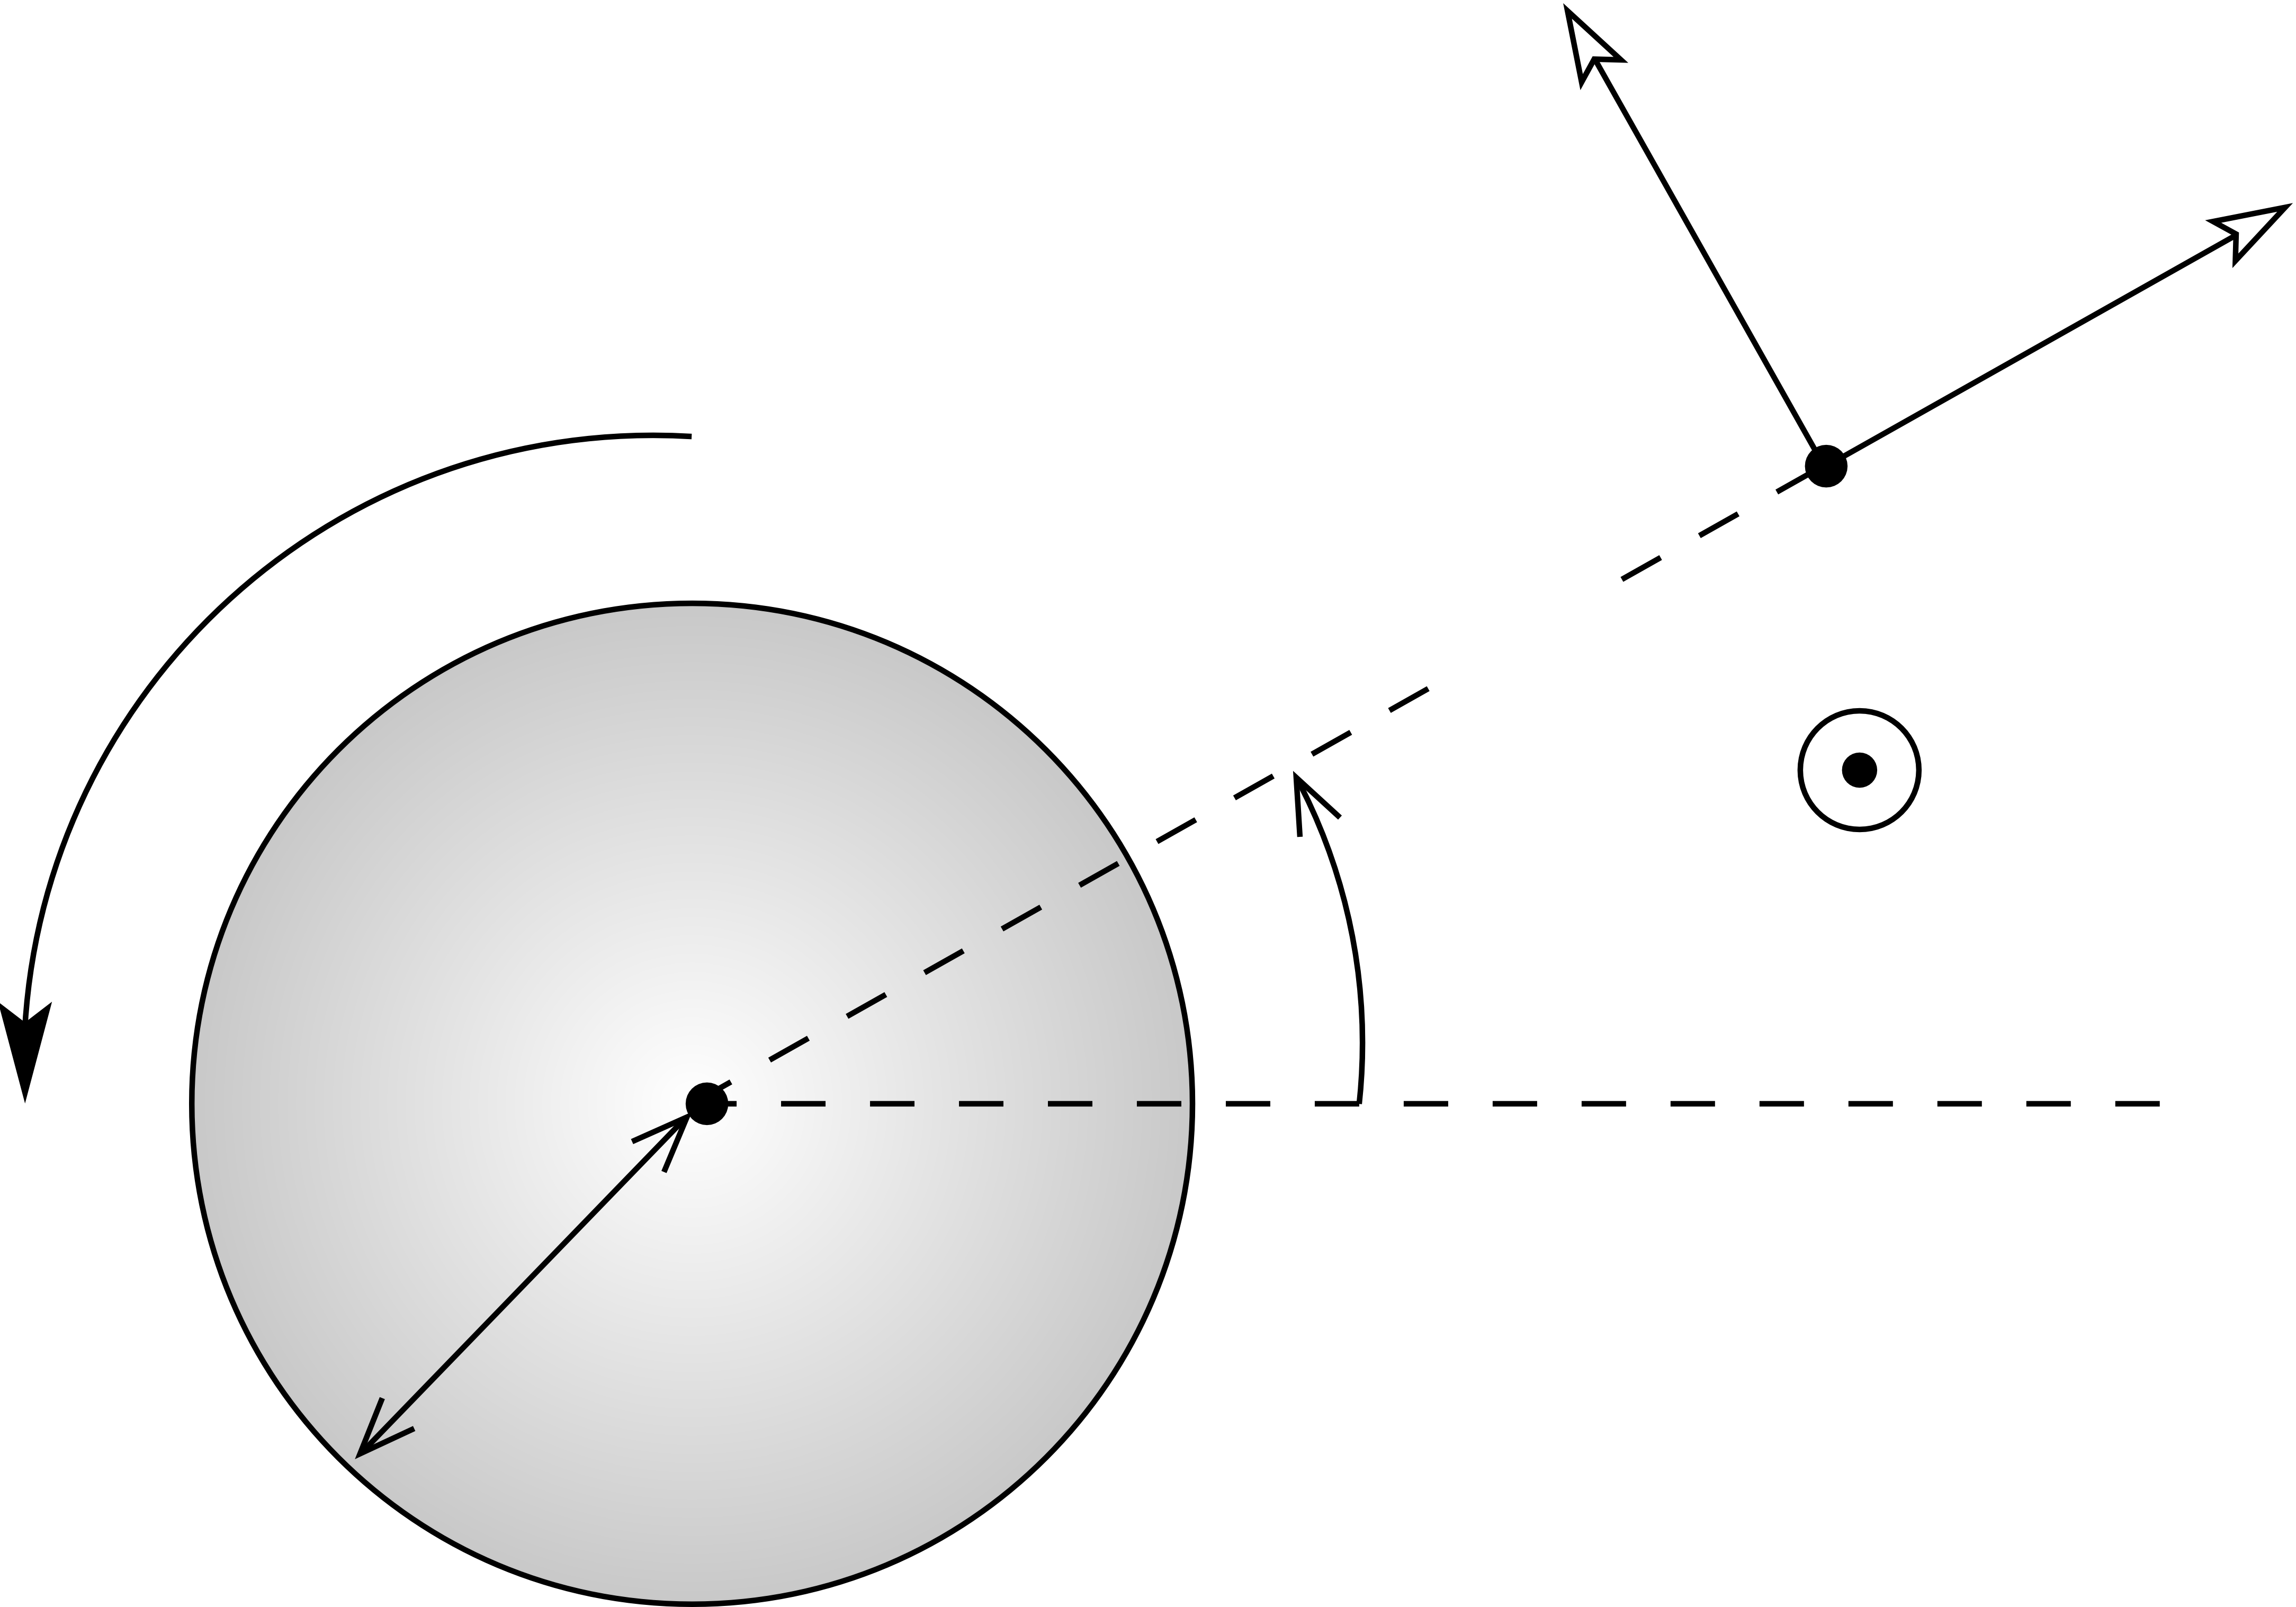
\includegraphics[width=7cm]{cylindre.png}}
\put(12, 10){$R$}
\put(5, 33){$\omega$}
\put(19, 17){$O$}
\put(43, 20){$\theta$}
\put(46, 29){$r$}
\put(67, 37){$\mathbf{e}_r$}
\put(53, 45){$\mathbf{e}_\theta$}
\put(61, 25){$\mathbf{e}_z$}
\end{picture}
\end{center}
\caption{Cylindre en rotation}
\label{fig:cylindre_tournant}
\end{figure}


Le cylindre est reli\'e \`a un moteur qui, mis en route \`a $t=0$,
lui impose une vitesse angulaire constante $\omega$ (rad/s) autour
de son axe $Oz$ (fig.~\ref{fig:cylindre_tournant}).

\begin{enumerate}
\setcounter{enumi}{0}
\item
Expliquer en quelques mots pourquoi et comment le liquide initialement
au repos va se mettre en mouvement.
On précisera en particulier le mode de transport de la quantité de mouvement
impliqué. 
Imaginer les lignes de courant de l'\'ecoulement ainsi g\'en\'er\'e
(faire un dessin).
\item
Apr\`es un r\'egime transitoire de mise en mouvement du liquide,
l'\'ecoulement tend \`a devenir stationnaire dans le voisinage du cylindre.
Quel pourrait \^etre une premi\`ere approximation de l'ordre de grandeur
de la dur\'ee $\tau$ du r\'egime transitoire ? 
\end{enumerate}
\noindent
On s'int\'eresse dor\'enavant au r\'egime quasi permanent aux temps longs $t \gg \tau$.
On rappelle que les \'equations d'un \'ecoulement incompressible plan
en coordonn\'ees polaires 
$\mathbf{u} = u(r, \theta, t) \, \mathbf{e}_r + v(r, \theta, t) \, \mathbf{e}_\theta$
s'\'ecrivent
\begin{eqnarray}
              \frac{\partial u}{\partial t}
+           u \frac{\partial u}{\partial r}
+ \frac{v}{r} \frac{\partial u}{\partial \theta} - \frac{v^2}{r}
& = &
- \frac{1}{\,\rho\,} \frac{\partial p}{\partial r} \,
+ \nu \left [ 	
\frac{\partial}{\partial r} \left (\frac{1}{r} \frac{\partial}{\partial r} (ru)  \right )  
+ \frac{1}{r^2} \frac{\partial^2 u}{\partial \theta^2} 
- \frac{2}{r^2} \frac{\partial v}{\partial \theta}
\right ]
\\
              \frac{\partial v}{\partial t}
+           u \frac{\partial v}{\partial r}
+ \frac{v}{r} \frac{\partial v}{\partial \theta} + \frac{uv}{r}
& = &
- \frac{1}{\rho r} \frac{\partial p}{\partial \theta}
+ \nu \left [ 	
\frac{\partial}{\partial r} \left (\frac{1}{r} \frac{\partial}{\partial r} (rv)  \right )  
+ \frac{1}{r^2} \frac{\partial^2 v}{\partial \theta^2} 
+ \frac{2}{r^2} \frac{\partial u}{\partial \theta}
\right ]
\\
\frac{\partial}{\partial r}(ru) + \frac{\partial v}{\partial \theta} & = & 0
\end{eqnarray}
            

\begin{enumerate}
\setcounter{enumi}{2}
\item
Justifier bri\`evement pourquoi il est a priori l\'egitime de rechercher
une solution d'\'ecoulement purement azimutal et axisym\'etrique, 
de la forme $\mathbf{u} = v(r) \, \mathbf{e}_\theta$.
\item
En injectant ce type de solution dans les \'equations du mouvement,
montrer dans un premier temps que le champ de pression ne d\'epend
que de $r$.
\item
R\'esoudre l'\'equation diff\'erentielle v\'erifi\'ee par $v(r)$
en prenant en compte les conditions aux limites d'adh\'erence \`a la paroi
imperm\'eable du cylindre en rotation et de d\'ecroissance du champ
de vitesse loin du cylindre.
\item
Montrer qu'il s'agit d'un \'ecoulement irrotationnel.
On rappelle que le rotationnel en cylindriques pour un champ bidimensionnel
$\mathbf{F} = F_r(r, \theta) \, \mathbf{e}_r + F_\theta(r, \theta) \, \mathbf{e}_\theta$
se r\'eduit \`a
\[
\textbf{rot} \, \mathbf{F} = \frac{1}{r} \left [ 
\frac{\partial}{\partial r}(rF_\theta) - \frac{\partial F_r}{\partial \theta}
\right ] \, \mathbf{e}_z
\]
\item
Calculer le champ de pression $p(r)$.
On notera $P_0$ la pression loin du cylindre.
\label{question:pression}
\end{enumerate}
\noindent
Bien que le terme visqueux $\nu \boldsymbol{\Delta} \mathbf{u}$ soit nul pour cet
\'ecoulement, ce n'est pas le cas pour les contraintes visqueuses au sein du fluide.
On rappelle que le tenseur des contraintes en coordonn\'ees polaires s'\'ecrit :
\begin{equation*}
\stackrel{\Rightarrow}{\sigma} =
\left (
\begin{array}{cc}
\sigma_{rr}      & \sigma_{r\theta} \\
\sigma_{r\theta} & \sigma_{\theta\theta}
\end{array}
\right ) 
\; \mbox{avec} \;
\sigma_{rr} = -p + 2\mu \frac{\partial u}{\partial r}, \;
\sigma_{\theta\theta} = -p + 2\mu 	\left (
	\frac{1}{r} \frac{\partial v}{\partial \theta} 
      + \frac{\partial u}{\partial r} 	\right ), \;
\sigma_{r\theta} = \mu \left (
  	\frac{1}{r} \frac{\partial u}{\partial \theta} 
      + \frac{\partial v}{\partial r}
      - \frac{v}{r}    \right )
\end{equation*}
\begin{enumerate}
\setcounter{enumi}{7}
\item
Calculer le tenseur $\stackrel{\Rightarrow}{\tau}$ des contraintes \textsl{visqueuses}.
\item
D\'eterminer la force \'el\'ementaire $d\mathbf{f}$ exerc\'ee
par le fluide sur un \'el\'ement de surface $dS$ de la paroi du cylindre.
\item
Donner l'expression du moment en $O$, not\'e $d\mathbf{M}_O$, de cette force \'el\'ementaire
puis du moment \textsl{r\'esultant} en $O$, not\'e $\mathbf{M}_O$, de la force de
frottement exerc\'ee par le fluide sur toute la surface du cylindre.
\item
En d\'eduire le couple $\mathbf{C}$ que devrait imposer le moteur au cylindre
pour maintenir la rotation \`a vitesse angulaire $\omega$ constante.
Quelle est la puissance dissip\'ee $\cal P$ ? 
\end{enumerate}

\paragraph{Questions complémentaires :}
Le liquide dans lequel est plong\'e le cylindre poss\`ede une surface libre
avec l'air ext\'erieur \`a pression atmosph\'erique $P_{atm}$.
Au repos (cylindre immobile) cette surface se trouve \`a l'altitude $z = h_0$. 
On cherche ici \`a pr\'edire comment la mise en mouvement du cylindre
va d\'eformer cette surface libre.
Le champ de vitesse d\'etermin\'e pr\'ec\'edemment n'est pas modifi\'e
et conserve la m\^eme expression $v(r)$.
Ce n'est pas le cas pour le champ de pression, qu'il faut recalculer
en notant que la d\'ependance de la pression suivant la verticale est
maintenant affect\'ee par la prise en compte de la pesanteur:
\[
\frac{\partial p}{\partial z} = -g
\]
\begin{enumerate}
\setcounter{enumi}{11}
\item
Reprendre la question~\ref{question:pression} pour calculer le champ
de pression $p(r, z)$ dans le liquide.
\item
En négligeant les effets de tension de surface, d\'eterminer 
la forme de la surface libre $z=h(r)$.
Tracer qualitativement la forme de surface libre.
\end{enumerate}

On cherche pour finir \`a d\'eterminer l'influence d'un
cylindre ext\'erieur sur le couple \`a imposer au cylindre
principal pour le maintenir \`a vitesse angulaire constante $\omega$.
On consid\`ere donc que le liquide est confin\'e entre le cylindre principal
de rayon $R$ et un second cylindre \textit{immobile} de rayon $R^\star > R$.

\begin{enumerate}
\setcounter{enumi}{13}
\item
Reprendre les questions 3 \`a 5 pour calculer le champ de vitesse $v^\star(r)$.
\item
Calculer la contrainte visqueuse exerc\'ee par le liquide sur la paroi du
cylindre principal et en d\'eduire que le moment r\'esultant en $O$ par unit\'e
de longueur du frottement visqueux sur le cylindre est de la forme
\[
\mathbf{M}_O^\star = -4\pi \mu^\star \omega R^2 \, \mathbf{e}_z
\]
o\`u $\mu^\star$ est une fonction de $\mu$, $r$ et $R^\star$ \`a d\'eterminer. 
\item
Comparer le couple qu'il faut imposer ici pour maintenir une vitesse angulaire
$\omega$ constante par rapport au cas pr\'ec\'edent o\`u le second cylindre
est absent.
\end{enumerate}




